% Options for packages loaded elsewhere
\PassOptionsToPackage{unicode}{hyperref}
\PassOptionsToPackage{hyphens}{url}
\PassOptionsToPackage{dvipsnames,svgnames,x11names}{xcolor}
%
\documentclass[
  letterpaper,
  DIV=11,
  numbers=noendperiod]{scrartcl}

\usepackage{amsmath,amssymb}
\usepackage{iftex}
\ifPDFTeX
  \usepackage[T1]{fontenc}
  \usepackage[utf8]{inputenc}
  \usepackage{textcomp} % provide euro and other symbols
\else % if luatex or xetex
  \usepackage{unicode-math}
  \defaultfontfeatures{Scale=MatchLowercase}
  \defaultfontfeatures[\rmfamily]{Ligatures=TeX,Scale=1}
\fi
\usepackage{lmodern}
\ifPDFTeX\else  
    % xetex/luatex font selection
\fi
% Use upquote if available, for straight quotes in verbatim environments
\IfFileExists{upquote.sty}{\usepackage{upquote}}{}
\IfFileExists{microtype.sty}{% use microtype if available
  \usepackage[]{microtype}
  \UseMicrotypeSet[protrusion]{basicmath} % disable protrusion for tt fonts
}{}
\makeatletter
\@ifundefined{KOMAClassName}{% if non-KOMA class
  \IfFileExists{parskip.sty}{%
    \usepackage{parskip}
  }{% else
    \setlength{\parindent}{0pt}
    \setlength{\parskip}{6pt plus 2pt minus 1pt}}
}{% if KOMA class
  \KOMAoptions{parskip=half}}
\makeatother
\usepackage{xcolor}
\setlength{\emergencystretch}{3em} % prevent overfull lines
\setcounter{secnumdepth}{-\maxdimen} % remove section numbering
% Make \paragraph and \subparagraph free-standing
\ifx\paragraph\undefined\else
  \let\oldparagraph\paragraph
  \renewcommand{\paragraph}[1]{\oldparagraph{#1}\mbox{}}
\fi
\ifx\subparagraph\undefined\else
  \let\oldsubparagraph\subparagraph
  \renewcommand{\subparagraph}[1]{\oldsubparagraph{#1}\mbox{}}
\fi


\providecommand{\tightlist}{%
  \setlength{\itemsep}{0pt}\setlength{\parskip}{0pt}}\usepackage{longtable,booktabs,array}
\usepackage{calc} % for calculating minipage widths
% Correct order of tables after \paragraph or \subparagraph
\usepackage{etoolbox}
\makeatletter
\patchcmd\longtable{\par}{\if@noskipsec\mbox{}\fi\par}{}{}
\makeatother
% Allow footnotes in longtable head/foot
\IfFileExists{footnotehyper.sty}{\usepackage{footnotehyper}}{\usepackage{footnote}}
\makesavenoteenv{longtable}
\usepackage{graphicx}
\makeatletter
\def\maxwidth{\ifdim\Gin@nat@width>\linewidth\linewidth\else\Gin@nat@width\fi}
\def\maxheight{\ifdim\Gin@nat@height>\textheight\textheight\else\Gin@nat@height\fi}
\makeatother
% Scale images if necessary, so that they will not overflow the page
% margins by default, and it is still possible to overwrite the defaults
% using explicit options in \includegraphics[width, height, ...]{}
\setkeys{Gin}{width=\maxwidth,height=\maxheight,keepaspectratio}
% Set default figure placement to htbp
\makeatletter
\def\fps@figure{htbp}
\makeatother

\KOMAoption{captions}{tableheading}
\usepackage{fontspec}
\setmainfont{Times New Roman}
\usepackage{setspace}
\setstretch{1.25}
\fontsize{9pt}{12pt}\selectfont
\makeatletter
\makeatother
\makeatletter
\makeatother
\makeatletter
\@ifpackageloaded{caption}{}{\usepackage{caption}}
\AtBeginDocument{%
\ifdefined\contentsname
  \renewcommand*\contentsname{Table of contents}
\else
  \newcommand\contentsname{Table of contents}
\fi
\ifdefined\listfigurename
  \renewcommand*\listfigurename{List of Figures}
\else
  \newcommand\listfigurename{List of Figures}
\fi
\ifdefined\listtablename
  \renewcommand*\listtablename{List of Tables}
\else
  \newcommand\listtablename{List of Tables}
\fi
\ifdefined\figurename
  \renewcommand*\figurename{Figure}
\else
  \newcommand\figurename{Figure}
\fi
\ifdefined\tablename
  \renewcommand*\tablename{Table}
\else
  \newcommand\tablename{Table}
\fi
}
\@ifpackageloaded{float}{}{\usepackage{float}}
\floatstyle{ruled}
\@ifundefined{c@chapter}{\newfloat{codelisting}{h}{lop}}{\newfloat{codelisting}{h}{lop}[chapter]}
\floatname{codelisting}{Listing}
\newcommand*\listoflistings{\listof{codelisting}{List of Listings}}
\makeatother
\makeatletter
\@ifpackageloaded{caption}{}{\usepackage{caption}}
\@ifpackageloaded{subcaption}{}{\usepackage{subcaption}}
\makeatother
\makeatletter
\@ifpackageloaded{tcolorbox}{}{\usepackage[skins,breakable]{tcolorbox}}
\makeatother
\makeatletter
\@ifundefined{shadecolor}{\definecolor{shadecolor}{rgb}{.97, .97, .97}}
\makeatother
\makeatletter
\makeatother
\makeatletter
\makeatother
\ifLuaTeX
  \usepackage{selnolig}  % disable illegal ligatures
\fi
\IfFileExists{bookmark.sty}{\usepackage{bookmark}}{\usepackage{hyperref}}
\IfFileExists{xurl.sty}{\usepackage{xurl}}{} % add URL line breaks if available
\urlstyle{same} % disable monospaced font for URLs
\hypersetup{
  pdftitle={Walmart weekly sales mid-term project},
  pdfauthor={Yingmai Chen},
  colorlinks=true,
  linkcolor={blue},
  filecolor={Maroon},
  citecolor={Blue},
  urlcolor={Blue},
  pdfcreator={LaTeX via pandoc}}

\title{Walmart weekly sales mid-term project}
\author{Yingmai Chen}
\date{}

\begin{document}
\maketitle
\ifdefined\Shaded\renewenvironment{Shaded}{\begin{tcolorbox}[frame hidden, sharp corners, boxrule=0pt, borderline west={3pt}{0pt}{shadecolor}, interior hidden, breakable, enhanced]}{\end{tcolorbox}}\fi

\hypertarget{i.abstract}{%
\section{I.Abstract}\label{i.abstract}}

The project aims to find the relationship between weekly sales of
walmart with other variables,and the project will include six
parts:``Abstract'',``Introduction'',``method'',``results'',``discussion'',``appendix''.
The first two parts are the descriptions of this project,and the method
part would have two parts:EDA(Exploratory Data Analysis)which include
some visualization of my data and description of it,and for the model
part,it will include the formula of my model and some analysis of the
model,I plan to make six model.The results would be the comparison of
the model,like among these six model,which one I think is
best.Discussion part would discuss what should be improved about the
final model I choose,and some future questions about my project,appendix
would include some poorly visualized graphs when I do eda,so I don't
want to put it in eda part.

\hypertarget{ii.introduction}{%
\section{II.Introduction}\label{ii.introduction}}

In this study, we leveraged a dataset from Kaggle to identify and
quantify various factors impacting weekly sales. The dataset includes
key variables such as holidays, oil prices, temperature, unemployment
rates, and the Consumer Price Index (CPI), we utilized regression
analysis to assess the relative impact of these variables on sales
volumes.Through this study, we hope to offer a more comprehensive and
accurate sales forecasting model, helping businesses better understand
market dynamics and make more effective business decisions.

\hypertarget{iii.method}{%
\section{III.Method}\label{iii.method}}

I check the summary of the data first and see there don't have NA's in
the data,so we don't need to deal with the missing value of data.

\hypertarget{eda}{%
\subsection{EDA}\label{eda}}

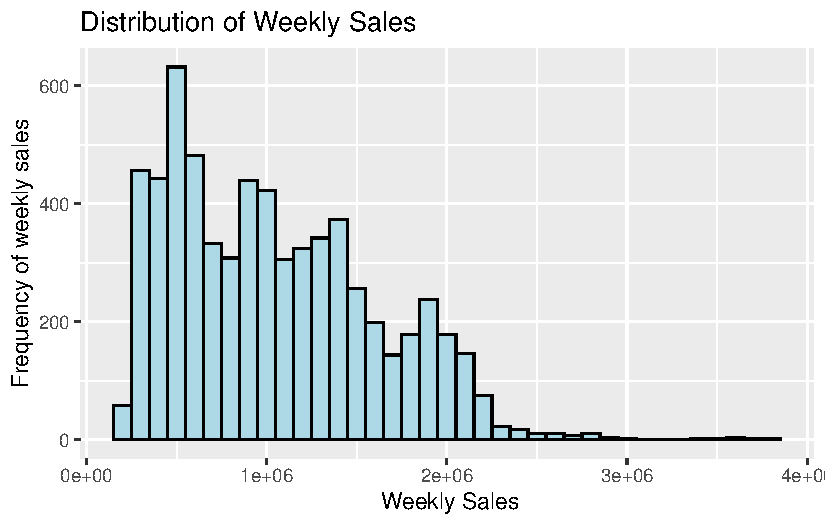
\includegraphics{678final_files/figure-pdf/distribution-plot-1.pdf}

\hypertarget{description}{%
\subsubsection{description}\label{description}}

From this plot,we can see that there are fewer weeks with very high
sales compared to weeks with low sales.This is typical for sales data
where a small number of periods (like holiday seasons) might have
exceptionally high sales.

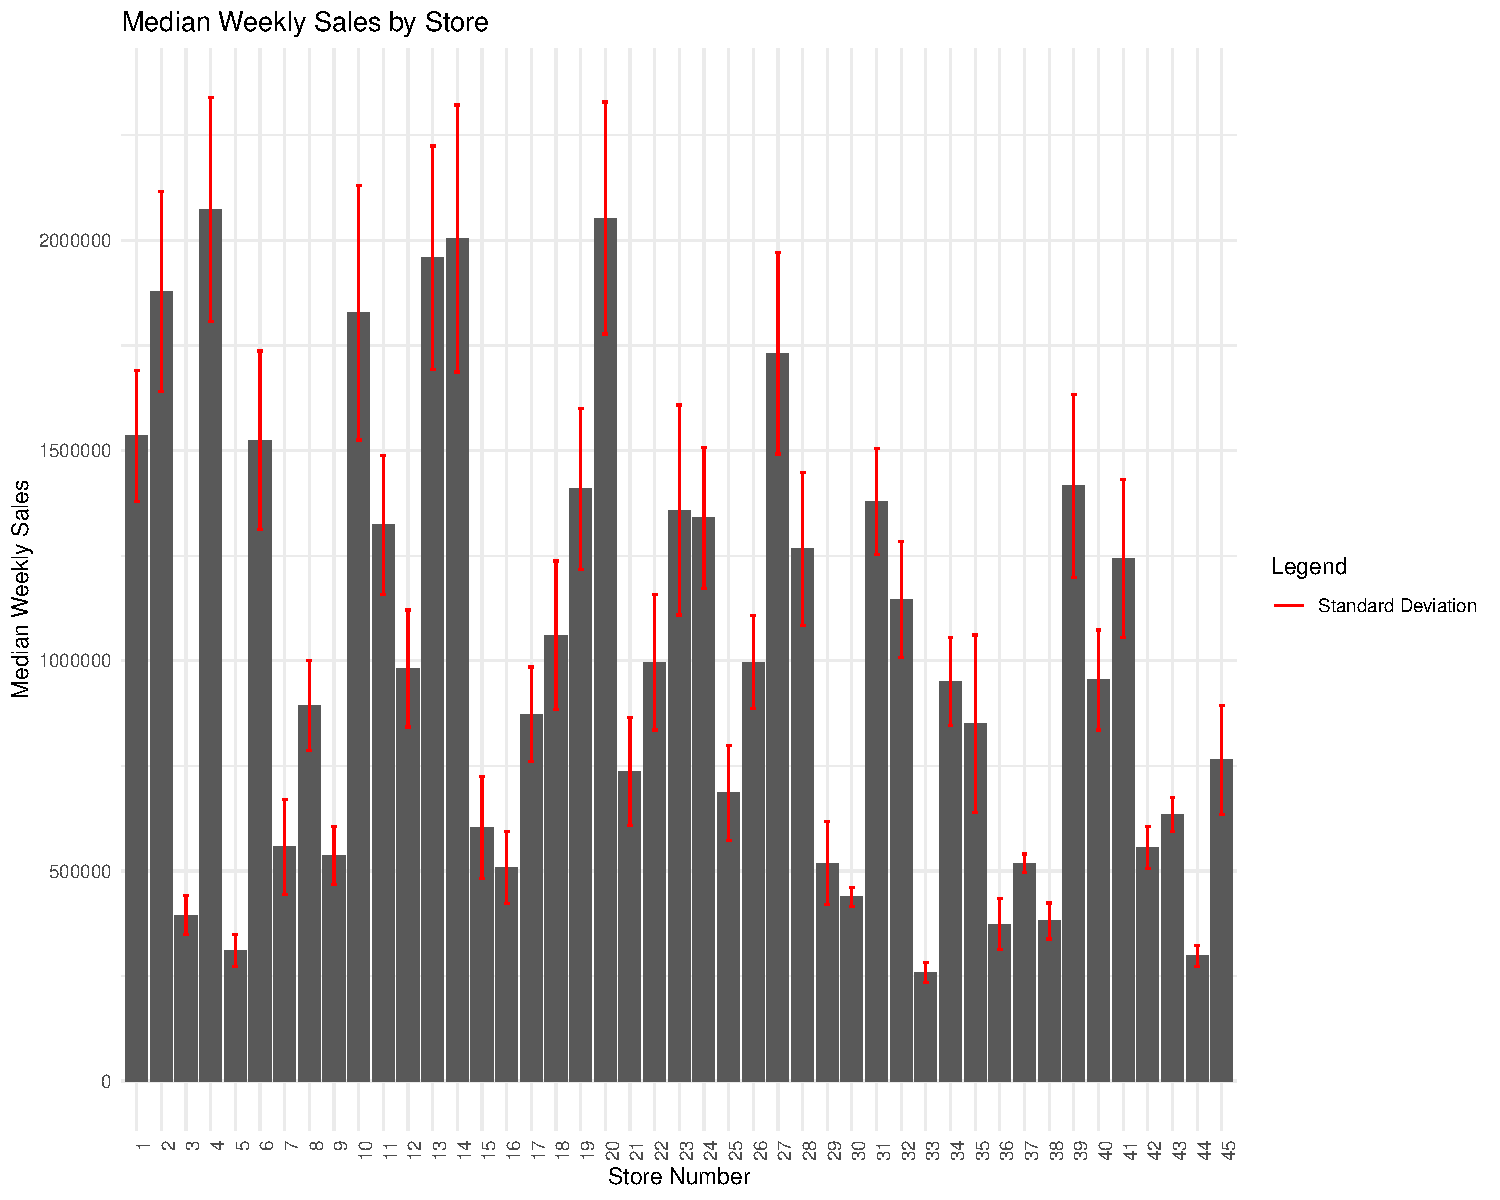
\includegraphics{678final_files/figure-pdf/bin-plot-1.pdf}

\hypertarget{description-1}{%
\subsubsection{description}\label{description-1}}

From this plot,we can see there exist obvious differences between each
store,some has higher median of weekly sales, and some would have bigger
error bar which means sales are more volatile.this suggests that we
should trying multilevel model in the model part.

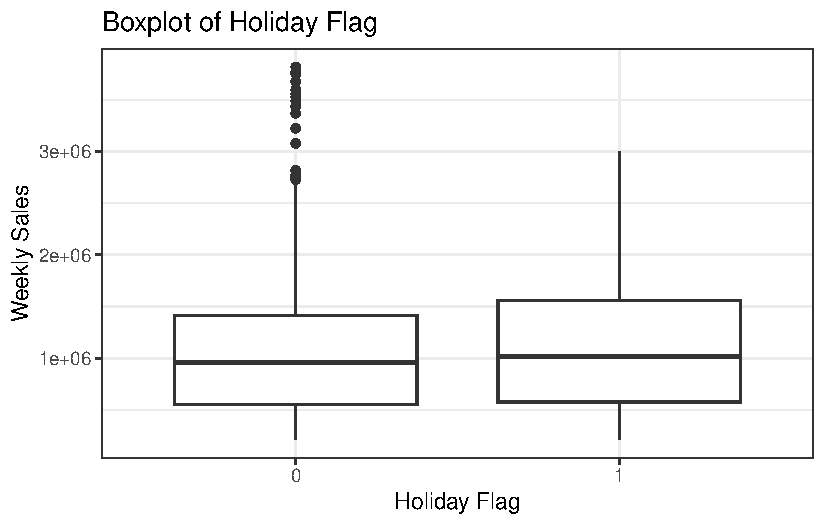
\includegraphics{678final_files/figure-pdf/box-plot-1.pdf}

\hypertarget{description-2}{%
\subsubsection{description}\label{description-2}}

From this plot, we can see that the median of holiday weekly sales is a
little bit higher than non-holiday weekly sale, and the numbers of
outliers in non-holiday weekly sales are more than holiday-weekly
sales,based on this,I think there would have some relationships between
holidays and weekly sales.

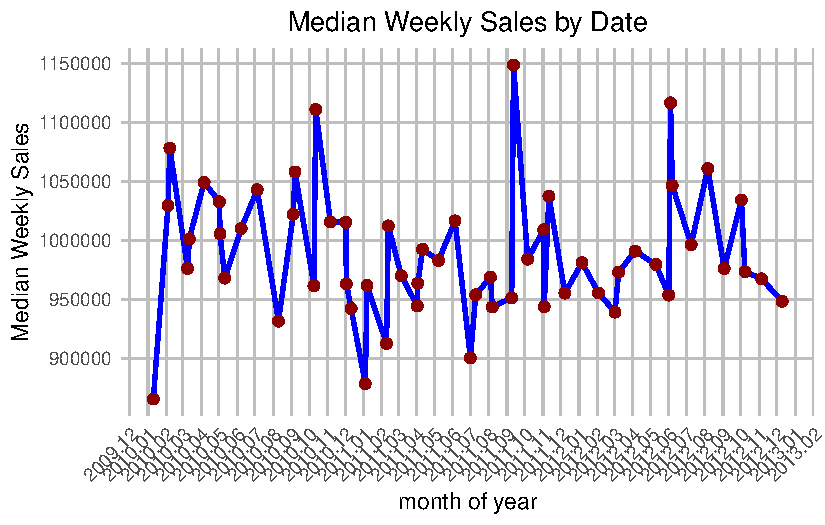
\includegraphics{678final_files/figure-pdf/line-plot-1.pdf}

\hypertarget{description-3}{%
\subsubsection{description}\label{description-3}}

From this plot,we can see that there is a recurring trend of lower sales
at the beginning of each year. This dip in sales could be attributed to
post-holiday season effects, where consumer spending typically drops
following the end-of-year holidays,which means the date would have
impact on weekly sales.

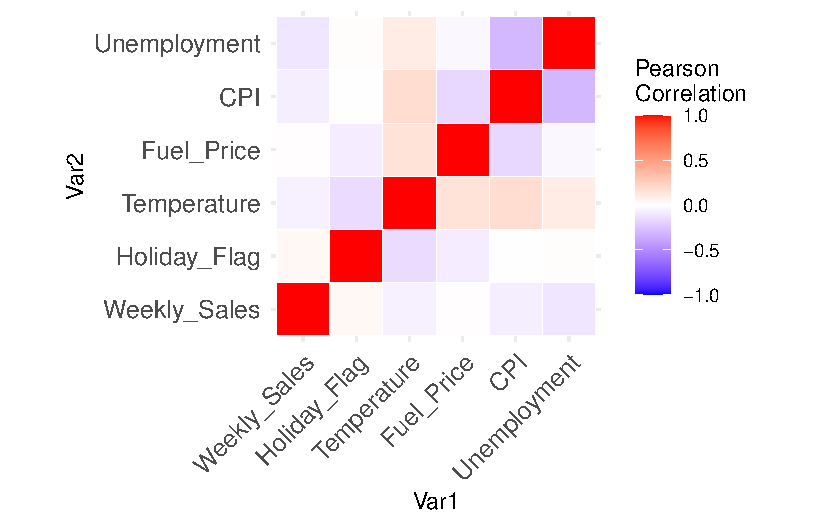
\includegraphics{678final_files/figure-pdf/matrix-plot-1.pdf}

\hypertarget{description-4}{%
\subsubsection{description}\label{description-4}}

As we can see, from this plot,It is not obvious that these variables are
correlated to weekly sales.

\hypertarget{model}{%
\subsection{Model}\label{model}}

Because we can not easily draw a conclusion by doing EDA,so the next
step for us shoud be modeling,

\hypertarget{model1null-model}{%
\subsubsection{model1:null model}\label{model1null-model}}

\[Weeklysales = \beta_0 + \varepsilon_i\]

\[\beta_0\] is the intercept, which is the average sales over all
observations in the data.

\[\varepsilon_i\] is the error term for the i-th observation.

\hypertarget{analysis-of-model1}{%
\paragraph{analysis of model1}\label{analysis-of-model1}}

Intercept: The estimated intercept is 1,046,965 with a standard error of
7,035. This intercept represents the average weekly sales across all
stores and dates included in the dataset.

Residuals: The residuals' range from -836,979 to 277,1722, with the
interquartile range (IQR) from -493,615 (1st quartile) to 37,194 (3rd
quartile). The large range of residuals indicates there is considerable
variability in weekly sales that the null model (using only the mean)
does not capture. The median of the residuals is -86,219, suggesting
that the model may systematically overestimate the weekly sales.

Mean Squared Error (MSE):The provided image shows the Mean Squared Error
(MSE) of the null model, which is 318460187634.It illustrated that The
null model's high MSE indicates it fails to accurately predict weekly
sales, lacking explanatory variables. To improve, incorporating factors
like promotions, store attributes, and seasonality into a more complex
model is essential.

\hypertarget{model2simple-linear-modelcomplete-pooling-model}{%
\subsubsection{model2:simple linear model(complete pooling
model)}\label{model2simple-linear-modelcomplete-pooling-model}}

\[\log(\text{Weekly_Sales}) = \beta_0 + \beta_1 \text{Holiday_Flag} + \beta_2 \text{Temperature} + \beta_3 \text{Fuel_Price} + \beta_4 \text{CPI} + \beta_5 \text{Unemployment} + \epsilon\]

\hypertarget{analysis-of-model2}{%
\paragraph{analysis of model2}\label{analysis-of-model2}}

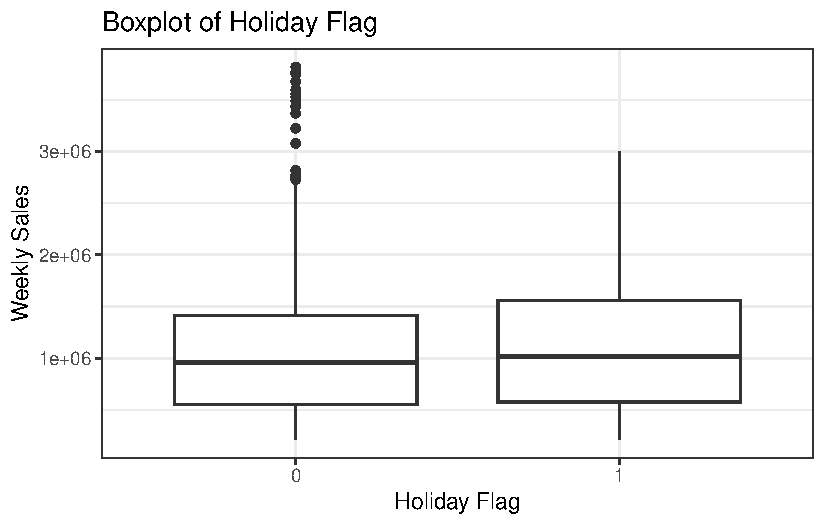
\includegraphics{678final_files/figure-pdf/unnamed-chunk-6-1.pdf}

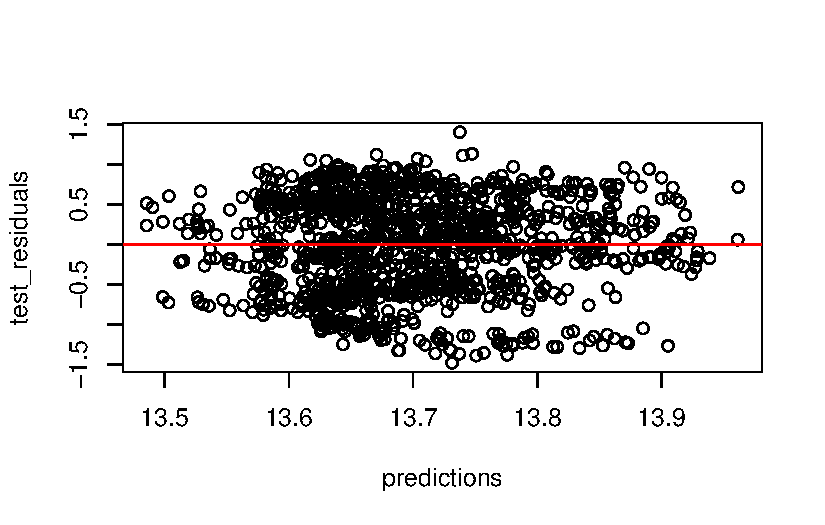
\includegraphics{678final_files/figure-pdf/unnamed-chunk-6-2.pdf}

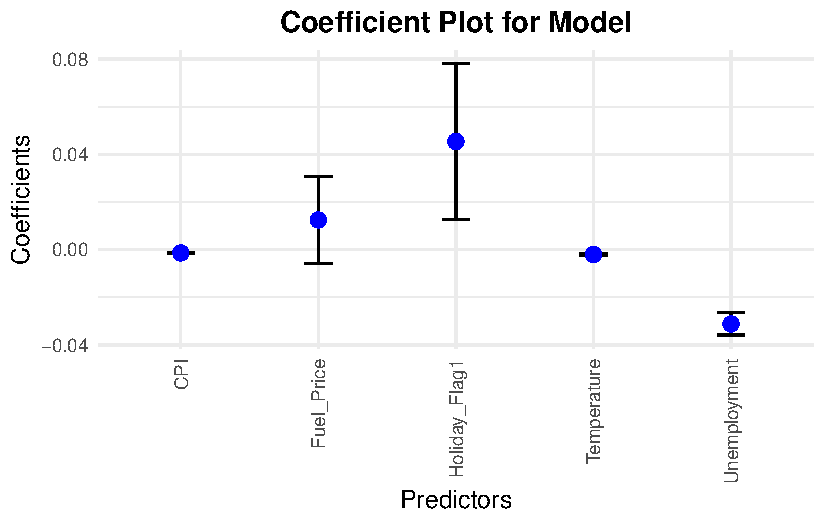
\includegraphics{678final_files/figure-pdf/unnamed-chunk-6-3.pdf}

The model has a very low R-squared value, indicating it does not explain
much of the variation in the data.Some predictors are statistically
significant, but given the low R-squared, their practical impact might
be limited. The assumptions of normality and homoscedasticity may be
violated based on the Q-Q plot and the Residuals vs.~Predictions plot,
which can affect the reliability of the model's standard errors and
p-values.There are outliers or extreme values that might be influencing
the results significantly.So all in all,simple linear model seems not to
be a good model to fit the data.

\hypertarget{model3multilevel-linear-model-with-random-intercept-no-pooling-model}{%
\subsubsection{model3:multilevel linear model with random intercept (No
pooling
model)}\label{model3multilevel-linear-model-with-random-intercept-no-pooling-model}}

\[\log(\text{Weekly_Sales}) = \beta_0 + \beta_1 \text{Temperature} + \beta_2 \text{Fuel_Price} + \beta_3 \text{CPI} + \beta_4 \text{Unemployment} + \beta_5 \text{Holiday_Flag} + u_j + \epsilon_i\]

\[\beta_0\] means the intercept term, representing the expected value of
the log sales when all other explanatory variables are zero.

\[u_j\] means andom effects term, capturing the effects introduced by
different stores (store j). This means each store has its own specific
impact (like location, size, customer base, etc.) that is not shared
with other stores.

\[\epsilon_i\] means error term.

So in this model,I will use the random value of intercept of store to
distinguish the different store.

\hypertarget{analysis-of-model3}{%
\paragraph{analysis of model3}\label{analysis-of-model3}}

\begin{verbatim}
Warning: 'r.squaredGLMM' now calculates a revised statistic. See the help page.
\end{verbatim}

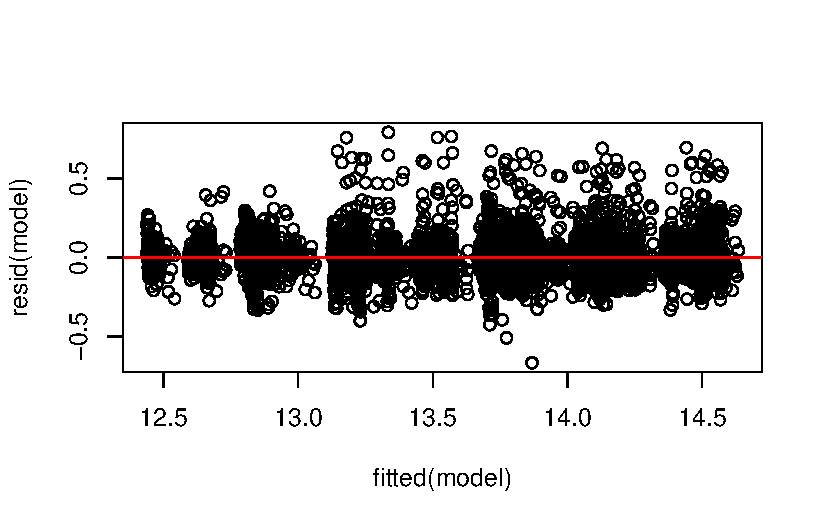
\includegraphics{678final_files/figure-pdf/unnamed-chunk-9-1.pdf}

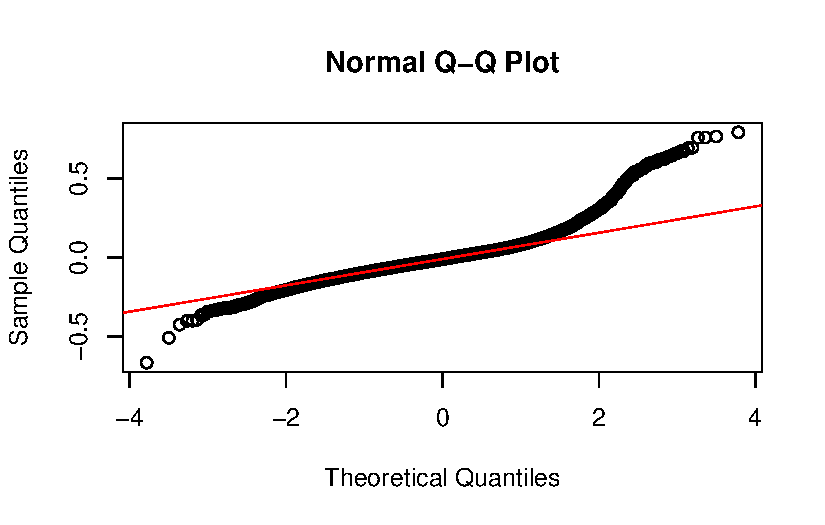
\includegraphics{678final_files/figure-pdf/unnamed-chunk-9-2.pdf}

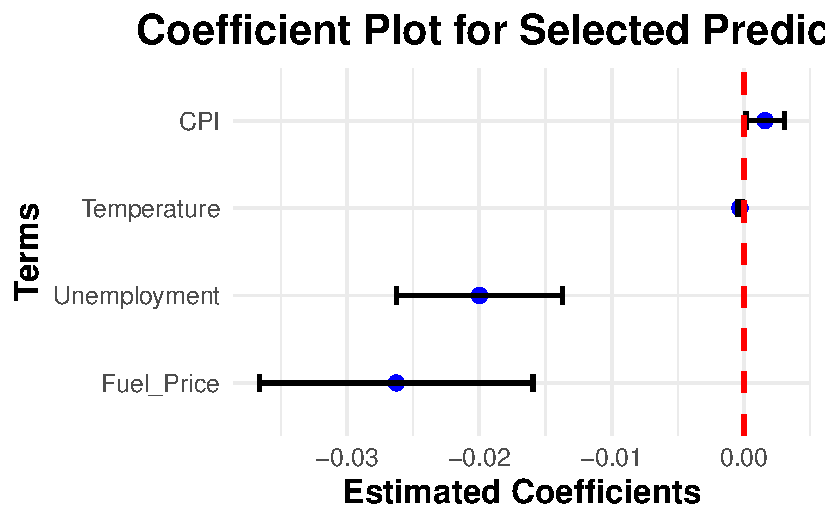
\includegraphics{678final_files/figure-pdf/unnamed-chunk-9-3.pdf}

Model Fit:

The conditional R-squared is extremely high, suggesting that when
accounting for both fixed and random effects, the model explains a large
proportion of the variance in sales.

The marginal R-squared is quite low, indicating that without the random
effects, the fixed effects do not explain much of the variance in sales.

Residual Diagnostics:

The residual plot does not show obvious patterns, which suggests that
the model does not suffer from non-linearity or heteroscedasticity
issues.

The QQ plot indicates deviations from normality, particularly in the
tails. This could point to issues with outlier responses or indicate
that the normal distribution may not be the best fit for the residuals.

In conclusion, while appears to be a good fit for capturing
store-to-store variation in sales, the fixed effects alone have limited
explanatory power.

\hypertarget{model4generalized-linear-modelcomplete-pooling}{%
\subsubsection{model4:generalized linear Model(complete
pooling)}\label{model4generalized-linear-modelcomplete-pooling}}

\[\log(\text{Weekly_Sales}) = \beta_0 + \beta_1 \text{Holiday_Flag} + \beta_2 \text{Temperature} + \beta_3 \text{Fuel_Price} + \beta_4 \text{CPI} + \beta_5 \text{Unemployment}\]

\hypertarget{analysis-of-model4}{%
\paragraph{analysis of model4}\label{analysis-of-model4}}

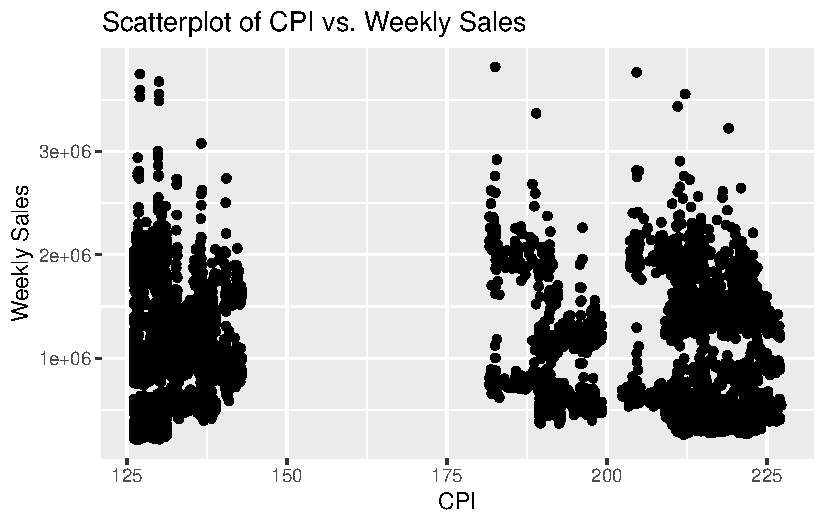
\includegraphics{678final_files/figure-pdf/unnamed-chunk-11-1.pdf}

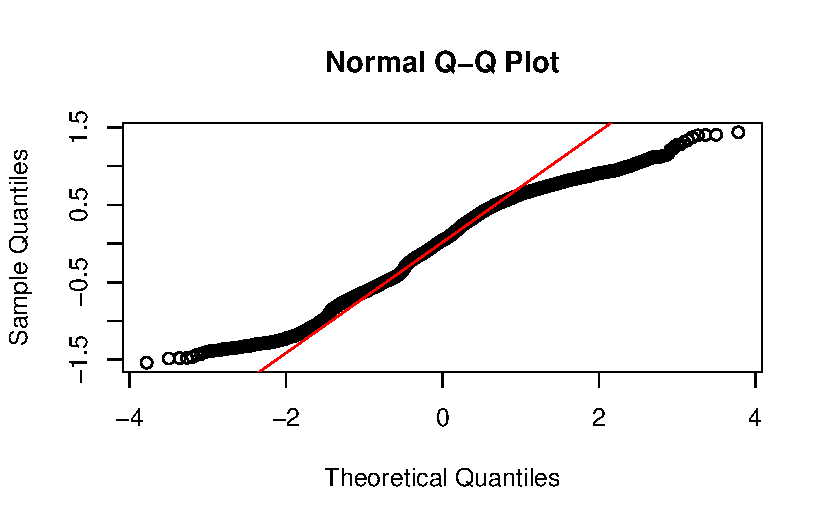
\includegraphics{678final_files/figure-pdf/unnamed-chunk-12-1.pdf}

After doing many analysis of this data,we find that it also shows a poor
fit with the data,Neither residual plot nor qq plot all shows it would
not fit to the data,so I decide not to do the no pooling anymore,I want
to try to improve model3 to make it fit better to the data.

\hypertarget{model5multilevel-generalized-linear-model-with-random-intercept-no-pooling}{%
\subsubsection{model5:multilevel generalized linear Model with random
intercept (No
pooling)}\label{model5multilevel-generalized-linear-model-with-random-intercept-no-pooling}}

\[\log(\text{Weekly_Sales}) = \beta_0 + \beta_1 \text{Temperature} + \beta_2 \text{Fuel_Price} + \beta_3 \text{CPI} + \beta_4 \text{Unemployment} + \beta_5 \text{Holiday_Flag} + u_j + \epsilon_i\]

\[\beta_0\] means the intercept term, representing the expected value of
the log sales when all other explanatory variables are zero.

\[u_j\] means andom effects term, capturing the effects introduced by
different stores (store j). This means each store has its own specific
impact (like location, size, customer base, etc.) that is not shared
with other stores.

\[\epsilon_i\] means error term.

\hypertarget{analysis-of-model5}{%
\paragraph{analysis of model5}\label{analysis-of-model5}}

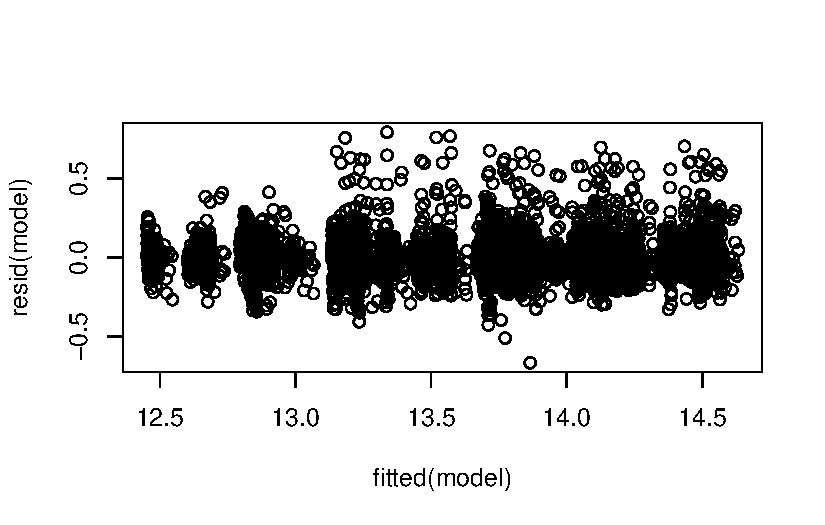
\includegraphics{678final_files/figure-pdf/unnamed-chunk-14-1.pdf}

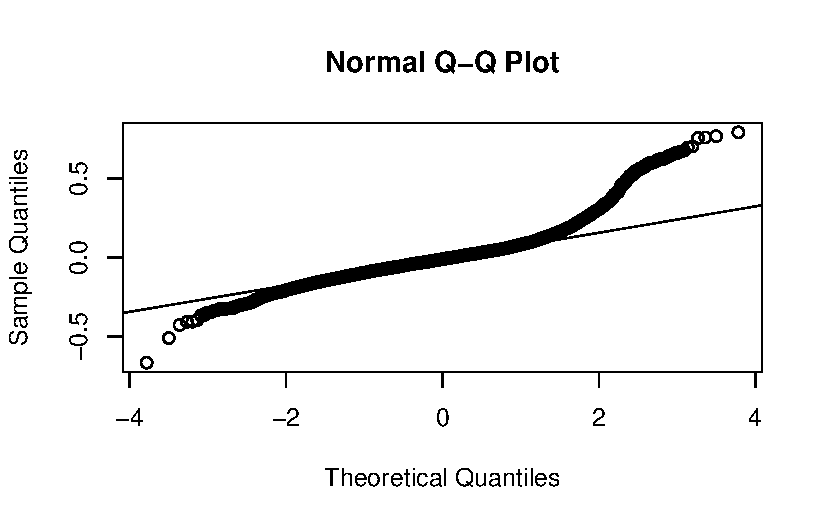
\includegraphics{678final_files/figure-pdf/unnamed-chunk-14-2.pdf}

From the qqplot ,we can see a deviation from the line in the tails,
suggesting that the residuals may not be normally distributed,
especially in the extremes. This could affect the validity of
statistical tests and confidence intervals.From the residual plot,we can
see a clear pattern of residuals, which is not ideal. We would prefer a
random scatter. The banding pattern could be due to discrete features in
the data or overdispersion.So it seems this model may not be a good
choice.

\hypertarget{model6multilevel-linear-model-with-random-coefficient-and-random-intercept-no-pooling}{%
\subsubsection{model6:multilevel linear Model with random coefficient
and random intercept (No
pooling)}\label{model6multilevel-linear-model-with-random-coefficient-and-random-intercept-no-pooling}}

\[\log(\text{Weekly_Sales}) = \alpha_{i} + \beta_{1[i]}\text{Temperature} + \beta_{2[i]}\text{Fuel_Price} + \beta_{3[i]}\text{CPI} + \beta_{4[i]}\text{Unemployment} + \beta_{5[i]}\text{Holiday_flag}+\epsilon_i\]

in this model,for \[\epsilon_i\],it means error term,\[\beta_{1[i]}\]
to\[\beta_{5[i]}\] means random coefficient of variables based on each
store and \[\alpha_{i}\] means random intercept.

\hypertarget{analysis-of-model6}{%
\paragraph{analysis of model6}\label{analysis-of-model6}}

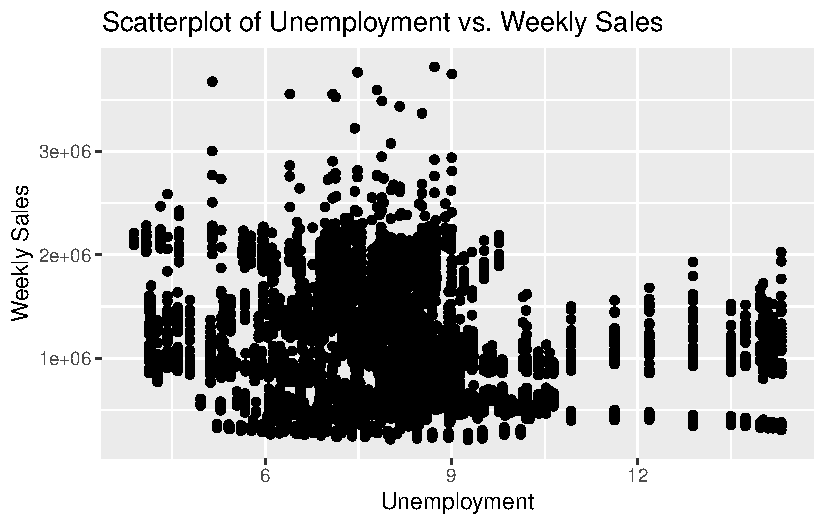
\includegraphics{678final_files/figure-pdf/unnamed-chunk-16-1.pdf}

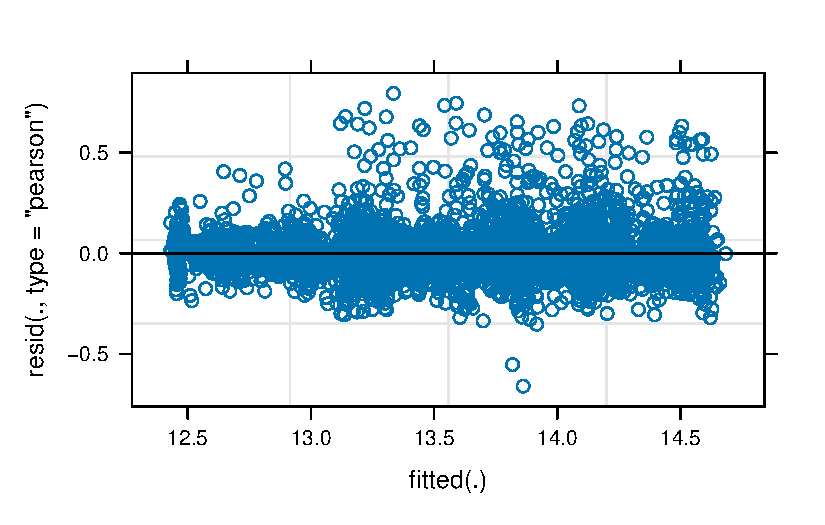
\includegraphics{678final_files/figure-pdf/unnamed-chunk-16-2.pdf}

From this qqplot,we can see some deviation from normality, especially in
the tails. This could affect the reliability of the p-values associated
with the fixed effects.From the residual plot, we can see it shows a
fairly random dispersion,besides,we also see the summary of the model,it
shows that the intercept and all predictors except for Temperature have
significant p-values, suggesting they contribute meaningfully to the
model.so based on these outputs, the model appears to be decent.

\hypertarget{iv.result}{%
\section{IV.result}\label{iv.result}}

I have mentioned in the abstract part,for the result part,what I want to
do is to choose from the six model I used to judge which one is the best
model,so among these six model,the first three should be exclude are the
null model,generalized linear Model,and the simple linear model,because
in the analysis part,we can see they all unsatisfactory,so for the last
part,what I will do is to make a competition between multilevel linear
Model with random coefficient and random intercept, multilevel linear
Model with random intercept,multilevel generalized linear Model with
random intercept.

\hypertarget{comparison}{%
\subsection{comparison}\label{comparison}}

\begin{verbatim}
Data: data
Models:
model3: Log_Weekly_Sales ~ Temperature + Fuel_Price + CPI + Unemployment + Holiday_Flag + (1 | Store)
model5: Log_Weekly_Sales ~ Temperature + Fuel_Price + CPI + Unemployment + Holiday_Flag + (1 | Store)
model6: Log_Weekly_Sales ~ Temperature + Fuel_Price + CPI + Unemployment + Holiday_Flag + (Temperature + Fuel_Price + CPI + Unemployment + Holiday_Flag | Store)
       npar     AIC     BIC logLik deviance  Chisq Df Pr(>Chisq)    
model3    8 -8590.2 -8536.0 4303.1  -8606.2                         
model5    8 -8757.1 -8703.0 4386.6  -8773.1 166.94  0               
model6   28 -9356.1 -9166.6 4706.1  -9412.1 639.01 20  < 2.2e-16 ***
---
Signif. codes:  0 '***' 0.001 '**' 0.01 '*' 0.05 '.' 0.1 ' ' 1
\end{verbatim}

model3 is multilevel linear Model with random intercept,model5 is
multilevel generalized linear Model with random intercept,model6 is
multilevel linear Model with random coefficient and random intercept.

AIC and BIC: model16 has the lowest AIC and BIC values, suggesting that
it fits the data best while considering model complexity. AIC and BIC
are fit indices that penalize for complexity, with lower values
typically indicating a model that fits well with fewer parameters.

Log-Likelihood: model16 has the highest log-likelihood value, which
indicates the most accurate fit to the data.

Significance Testing: The p-value for the Chisq statistic is well below
0.001, indicating that model16 represents a statistically significant
improvement over the other models.

Combining these insights, model16 appears to be the relatively best
model among the three. It not only provides the best fit to the data
(based on AIC, BIC, and log-likelihood) but also accounts for model
complexity in a penalized manner. Although this model is more complex
(as it includes random slopes), its ability to improve the fit seems to
outweigh the costs of increased complexity. Therefore, if the data
supports a more complex model structure and predictive ability is an
important consideration, model16 would be the better choice.

\hypertarget{v.discussion}{%
\section{V.discussion}\label{v.discussion}}

For the discussion part,I have mentioned in the abstract part,I will
point out some limitation of multilevel linear Model with random
coefficient and random intercept(model I choose) and future questions.

\hypertarget{limitation}{%
\subsection{limitation}\label{limitation}}

For the predictor Significance temperature is insignificance (p
\textgreater{} 0.05),which suggests it may not be an important predictor
for \texttt{Log\_Weekly\_Sales} within this model, potentially limiting
the model's explanatory power regarding the influence of temperature on
sales. For the qqplot part, deviations from normality, particularly in
the tails as shown by the Q-Q plot, question the reliability of the
model's p-values and confidence intervals, impacting the validity of
statistical inferences.Foe r the residual plot,the funnel pattern
observed in the residuals versus fitted values plot indicates the
presence of heteroscedasticity, which means that the error variance is
not constant. This can affect the efficiency of the estimators and the
predictive performance of the model.

\hypertarget{future-questions}{%
\subsection{future questions}\label{future-questions}}

For the future question,I think first we should further investigate the
Temperature variable to see if there is a nonlinear relationship or
interactions with other variables that are not captured in the current
model. And we should try to explore more complex random effects
structures to better capture the variability in the data, such as
including random slopes for certain predictors.

\hypertarget{vi.appendix}{%
\section{VI.appendix}\label{vi.appendix}}

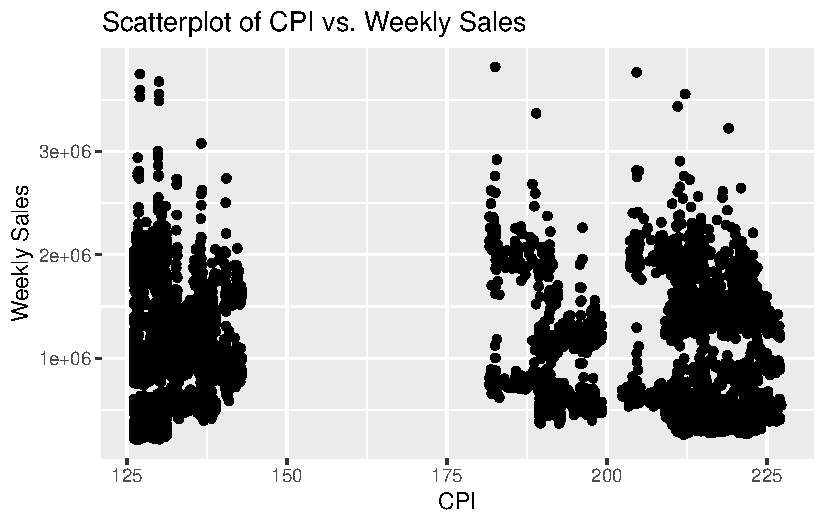
\includegraphics{678final_files/figure-pdf/unnamed-chunk-18-1.pdf}

From this plot, we can hardly see if there exist relationships between
CPI and weekly sales.

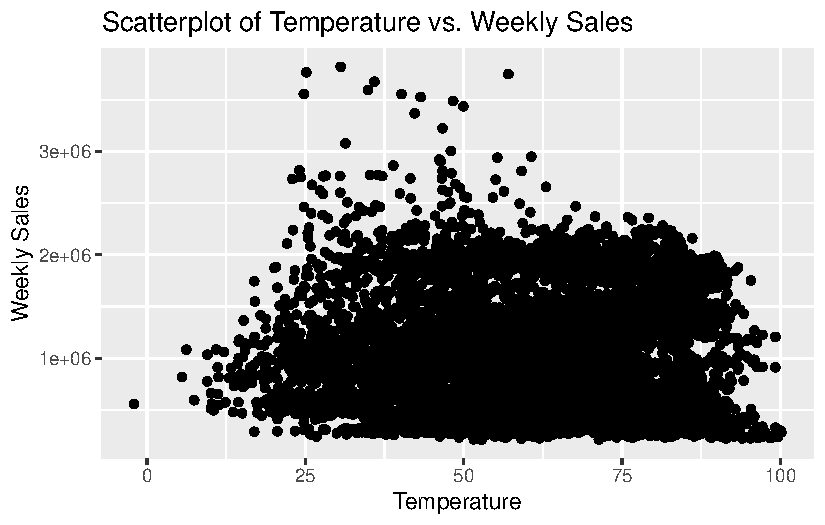
\includegraphics{678final_files/figure-pdf/unnamed-chunk-19-1.pdf}

From this plot,we can see temperatures from 25 to 75 of the country tend
to have much more numbers of higher weekly sales.

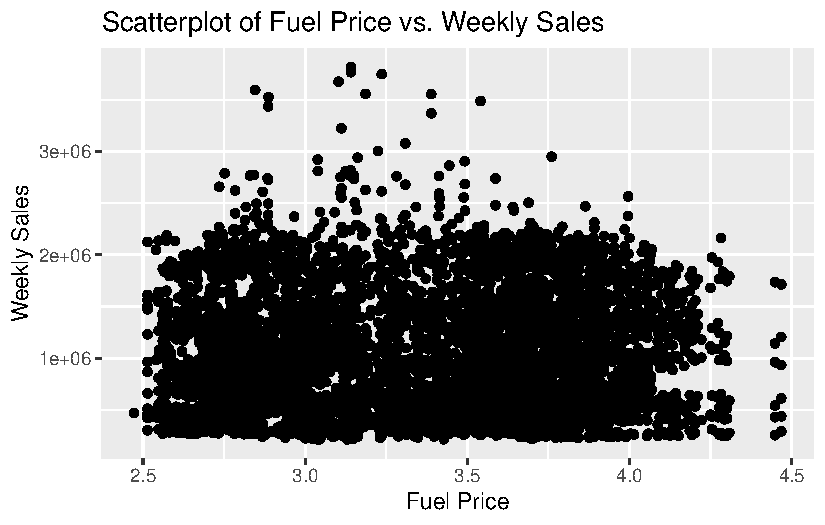
\includegraphics{678final_files/figure-pdf/unnamed-chunk-20-1.pdf}

From this plot, we can hardly see if there exist relationships between
fuel price and weekly sales.

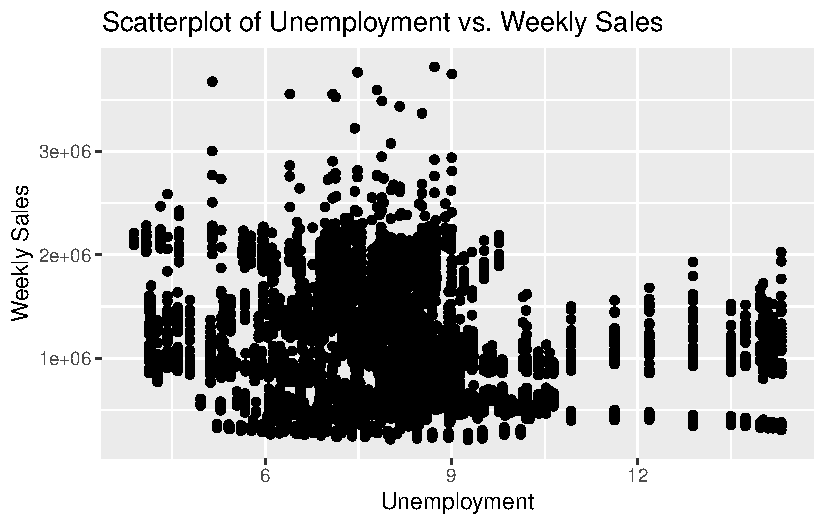
\includegraphics{678final_files/figure-pdf/unnamed-chunk-21-1.pdf}

From this plot,we can see the less of proportions of unemployment tends
to have higher weekly sales.



\end{document}
